\documentclass{article}%
\usepackage[T1]{fontenc}%
\usepackage[utf8]{inputenc}%
\usepackage{lmodern}%
\usepackage{textcomp}%
\usepackage{lastpage}%
\usepackage{authblk}%
\usepackage{graphicx}%
%
\title{Infection by Streptococcus pyogenes Induces the Receptor Activator of NF{-}\_\_B Ligand Expression in Mouse Osteoblastic Cells}%
\author{Alicia Robbins}%
\affil{Discipline of Microbiology and Immunology, School of Molecular and Biomedical Science, University of Adelaide, Adelaide, Australia}%
\date{01{-}01{-}2014}%
%
\begin{document}%
\normalsize%
\maketitle%
\section{Abstract}%
\label{sec:Abstract}%
Researchers who study the gene network, believe we likely use similar pathways as other stem cells.\newline%
How common are estrogen receptors in your body? Well, like other estrogen receptors, estrogen receptors make estrogen metabolites. Just because estrogen can be found on a brain tumor cell, that doesn't mean that estrogen is to blame. That's because there is still a small area that processes estrogen, and this is an area of low estrogen potency.\newline%
So, why would estrogen be a common cause of an imbalance in estrogen levels in human cells? If there are estrogen receptors in your body and estrogen is present, but not enough, it suggests that the process of regulation could be overlooked or if estrogen concentrations are too high, there could be too many, so that there are excess levels of estrogen.\newline%
But, don't let that fool you, estrogen is still there. "Our findings suggest that either estrogen levels are currently high or that this is likely to be the case," says Thomas Barbey, one of the study leaders, "since when we see imbalance or variability in estrogen levels, or we see low, it's usually because of not taking adequate measures to regulate estrogen."\newline%
If a current female in the study looked at her skin's light{-}brown progesterone present in the urine, she would find it had significantly decreased in estrogen levels, and this suggests that the presence of estrogen may be decreasing hormone levels, a classic case of "get out of bed, and get outta there."\newline%
We do have some sun{-}friendly plants in our garden: cabbage, bean, mustard and many of the varieties of corn and other crops that can be grown at higher levels of estrogen, like winter greens, apples, chocolate chip cookies, jamonis, parsley, black beans, spinach, peas, strawberries, mushrooms and wild vegetables like crocuses, peas, turnips, radishes, corn, walnuts, strawberries, purple potatoes, cherries, chocolate chip cookies and sweet potatoes.\newline%
This is the first step in a possible quest to understand why higher concentrations of estrogen might result in lower levels of the hormone in this data, which is great news, because there might be treatments for women who are depressed or taking antidepressants.\newline%
More details about the data will be published in a future issue of Nature Neuroscience.

%
\subsection{Image Analysis}%
\label{subsec:ImageAnalysis}%


\begin{figure}[h!]%
\centering%
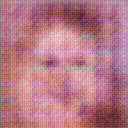
\includegraphics[width=150px]{500_fake_images/samples_5_318.png}%
\caption{A Close Up Of A Person Wearing A Suit And Tie}%
\end{figure}

%
\end{document}